% GNUPLOT: LaTeX picture with Postscript
\documentclass{minimal}
% Set font size
\makeatletter
\def\@ptsize{1}
\InputIfFileExists{size11.clo}{}{%
   \GenericError{(gnuplot) \space\space\space\@spaces}{%
      Gnuplot Error: File `size11.clo' not found! Could not set font size%
   }{See the gnuplot documentation for explanation.%
   }{For using a font size a file `size<fontsize>.clo' has to exist.
        Falling back ^^Jto default fontsize 10pt.}%
  \def\@ptsize{0}
  \input{size10.clo}%
}%
\makeatother
% Load packages
\usepackage{calc}
\usepackage{graphicx}
\usepackage{color}
\usepackage{transparent}
\makeatletter
% Select an appropriate default driver (from TeXLive graphics.cfg)
\begingroup
  \chardef\x=0 %
  % check pdfTeX
  \@ifundefined{pdfoutput}{}{%
    \ifcase\pdfoutput
    \else
      \chardef\x=1 %
    \fi
  }%
  % check VTeX
  \@ifundefined{OpMode}{}{%
    \chardef\x=2 %
  }%
\expandafter\endgroup
\ifcase\x
  % default case
  \PassOptionsToPackage{dvips}{geometry}
\or
  % pdfTeX is running in pdf mode
  \PassOptionsToPackage{pdftex}{geometry}
\else
  % VTeX is running
  \PassOptionsToPackage{vtex}{geometry}
\fi
\makeatother
% Set papersize
\usepackage[papersize={216.00bp,432.00bp},text={216.00bp,432.00bp}]{geometry}
% No page numbers and no paragraph indentation
\pagestyle{empty}
\setlength{\parindent}{0bp}%
% Load configuration file
\InputIfFileExists{gnuplot.cfg}{%
  \typeout{Using configuration file gnuplot.cfg}%
}{%
 \typeout{No configuration file gnuplot.cfg found.}%
}%
\usepackage[scaled]{helvet}\usepackage[T1]{fontenc}\renewcommand\familydefault{\sfdefault}\usepackage{amssymb,bm}\usepackage{siunitx}\usepackage[siunitx]{gnuplottex}\usepackage{xcolor}\definecolor{blue}{RGB}{0,114,178}\definecolor{red}{RGB}{213,94,0}\definecolor{yellow}{RGB}{240,228,66} \definecolor{green}{RGB}{0,158,115}\newcommand{\hl}[1]{\setlength{\fboxsep}{0.75pt}\colorbox{white}{#1}}\usepackage[fontsize=9pt]{fontsize}
\begin{document}
\begingroup
  \makeatletter
  \providecommand\color[2][]{%
    \GenericError{(gnuplot) \space\space\space\@spaces}{%
      Package color not loaded in conjunction with
      terminal option `colourtext'%
    }{See the gnuplot documentation for explanation.%
    }{Either use 'blacktext' in gnuplot or load the package
      color.sty in LaTeX.}%
    \renewcommand\color[2][]{}%
  }%
  \providecommand\includegraphics[2][]{%
    \GenericError{(gnuplot) \space\space\space\@spaces}{%
      Package graphicx or graphics not loaded%
    }{See the gnuplot documentation for explanation.%
    }{The gnuplot epslatex terminal needs graphicx.sty or graphics.sty.}%
    \renewcommand\includegraphics[2][]{}%
  }%
  \providecommand\rotatebox[2]{#2}%
  \@ifundefined{ifGPcolor}{%
    \newif\ifGPcolor
    \GPcolortrue
  }{}%
  \@ifundefined{ifGPblacktext}{%
    \newif\ifGPblacktext
    \GPblacktexttrue
  }{}%
  % define a \g@addto@macro without @ in the name:
  \let\gplgaddtomacro\g@addto@macro
  % define empty templates for all commands taking text:
  \gdef\gplbacktext{}%
  \gdef\gplfronttext{}%
  \makeatother
  \ifGPblacktext
    % no textcolor at all
    \def\colorrgb#1{}%
    \def\colorgray#1{}%
  \else
    % gray or color?
    \ifGPcolor
      \def\colorrgb#1{\color[rgb]{#1}}%
      \def\colorgray#1{\color[gray]{#1}}%
      \expandafter\def\csname LTw\endcsname{\color{white}}%
      \expandafter\def\csname LTb\endcsname{\color{black}}%
      \expandafter\def\csname LTa\endcsname{\color{black}}%
      \expandafter\def\csname LT0\endcsname{\color[rgb]{1,0,0}}%
      \expandafter\def\csname LT1\endcsname{\color[rgb]{0,1,0}}%
      \expandafter\def\csname LT2\endcsname{\color[rgb]{0,0,1}}%
      \expandafter\def\csname LT3\endcsname{\color[rgb]{1,0,1}}%
      \expandafter\def\csname LT4\endcsname{\color[rgb]{0,1,1}}%
      \expandafter\def\csname LT5\endcsname{\color[rgb]{1,1,0}}%
      \expandafter\def\csname LT6\endcsname{\color[rgb]{0,0,0}}%
      \expandafter\def\csname LT7\endcsname{\color[rgb]{1,0.3,0}}%
      \expandafter\def\csname LT8\endcsname{\color[rgb]{0.5,0.5,0.5}}%
    \else
      % gray
      \def\colorrgb#1{\color{black}}%
      \def\colorgray#1{\color[gray]{#1}}%
      \expandafter\def\csname LTw\endcsname{\color{white}}%
      \expandafter\def\csname LTb\endcsname{\color{black}}%
      \expandafter\def\csname LTa\endcsname{\color{black}}%
      \expandafter\def\csname LT0\endcsname{\color{black}}%
      \expandafter\def\csname LT1\endcsname{\color{black}}%
      \expandafter\def\csname LT2\endcsname{\color{black}}%
      \expandafter\def\csname LT3\endcsname{\color{black}}%
      \expandafter\def\csname LT4\endcsname{\color{black}}%
      \expandafter\def\csname LT5\endcsname{\color{black}}%
      \expandafter\def\csname LT6\endcsname{\color{black}}%
      \expandafter\def\csname LT7\endcsname{\color{black}}%
      \expandafter\def\csname LT8\endcsname{\color{black}}%
    \fi
  \fi
    \setlength{\unitlength}{0.0500bp}%
    \ifx\gptboxheight\undefined%
      \newlength{\gptboxheight}%
      \newlength{\gptboxwidth}%
      \newsavebox{\gptboxtext}%
    \fi%
    \setlength{\fboxrule}{0.5pt}%
    \setlength{\fboxsep}{1pt}%
    \definecolor{tbcol}{rgb}{1,1,1}%
\begin{picture}(4320.00,8640.00)%
    \gplgaddtomacro\gplbacktext{%
      \csname LTb\endcsname%%
      \put(686,6501){\makebox(0,0)[r]{\strut{}$0.5$}}%
      \csname LTb\endcsname%%
      \put(686,6892){\makebox(0,0)[r]{\strut{}$1.5$}}%
      \csname LTb\endcsname%%
      \put(686,7283){\makebox(0,0)[r]{\strut{}$2.5$}}%
      \csname LTb\endcsname%%
      \put(686,7674){\makebox(0,0)[r]{\strut{}$3.5$}}%
      \csname LTb\endcsname%%
      \put(686,8065){\makebox(0,0)[r]{\strut{}$4.5$}}%
      \csname LTb\endcsname%%
      \put(784,6131){\makebox(0,0){\strut{}$0$}}%
      \csname LTb\endcsname%%
      \put(1244,6131){\makebox(0,0){\strut{}$10$}}%
      \csname LTb\endcsname%%
      \put(1704,6131){\makebox(0,0){\strut{}$20$}}%
      \csname LTb\endcsname%%
      \put(2164,6131){\makebox(0,0){\strut{}$30$}}%
      \csname LTb\endcsname%%
      \put(2625,6131){\makebox(0,0){\strut{}$40$}}%
      \csname LTb\endcsname%%
      \put(3085,6131){\makebox(0,0){\strut{}$50$}}%
      \csname LTb\endcsname%%
      \put(3545,6131){\makebox(0,0){\strut{}$60$}}%
      \csname LTb\endcsname%%
      \put(4005,6131){\makebox(0,0){\strut{}$70$}}%
    }%
    \gplgaddtomacro\gplfronttext{%
      \csname LTb\endcsname%%
      \put(231,7185){\rotatebox{-270}{\makebox(0,0){\strut{}pressure (\si{\mega\pascal})}}}%
      \csname LTb\endcsname%%
      \put(2394,5869){\makebox(0,0){\strut{}distance (\si{\km})}}%
      \csname LTb\endcsname%%
      \put(2506,6901){\makebox(0,0)[r]{\strut{}ideal}}%
      \csname LTb\endcsname%%
      \put(2506,6551){\makebox(0,0)[r]{\strut{}non-ideal}}%
      \csname LTb\endcsname%%
      \put(2385,8327){\makebox(0,0){\strut{}(a)}}%
    }%
    \gplgaddtomacro\gplbacktext{%
      \csname LTb\endcsname%%
      \put(686,3684){\makebox(0,0)[r]{\strut{}$5$}}%
      \csname LTb\endcsname%%
      \put(686,4187){\makebox(0,0)[r]{\strut{}$15$}}%
      \csname LTb\endcsname%%
      \put(686,4689){\makebox(0,0)[r]{\strut{}$25$}}%
      \csname LTb\endcsname%%
      \put(686,5192){\makebox(0,0)[r]{\strut{}$35$}}%
      \csname LTb\endcsname%%
      \put(784,3258){\makebox(0,0){\strut{}$0$}}%
      \csname LTb\endcsname%%
      \put(1244,3258){\makebox(0,0){\strut{}$10$}}%
      \csname LTb\endcsname%%
      \put(1704,3258){\makebox(0,0){\strut{}$20$}}%
      \csname LTb\endcsname%%
      \put(2164,3258){\makebox(0,0){\strut{}$30$}}%
      \csname LTb\endcsname%%
      \put(2625,3258){\makebox(0,0){\strut{}$40$}}%
      \csname LTb\endcsname%%
      \put(3085,3258){\makebox(0,0){\strut{}$50$}}%
      \csname LTb\endcsname%%
      \put(3545,3258){\makebox(0,0){\strut{}$60$}}%
      \csname LTb\endcsname%%
      \put(4005,3258){\makebox(0,0){\strut{}$70$}}%
    }%
    \gplgaddtomacro\gplfronttext{%
      \csname LTb\endcsname%%
      \put(329,4312){\rotatebox{-270}{\makebox(0,0){\strut{}density (\si{\kilogram\per\cubic\meter})}}}%
      \csname LTb\endcsname%%
      \put(2394,2996){\makebox(0,0){\strut{}distance (\si{\km})}}%
      \csname LTb\endcsname%%
      \put(2506,4028){\makebox(0,0)[r]{\strut{}ideal}}%
      \csname LTb\endcsname%%
      \put(2506,3678){\makebox(0,0)[r]{\strut{}non-ideal}}%
      \csname LTb\endcsname%%
      \put(2385,5454){\makebox(0,0){\strut{}(b)}}%
    }%
    \gplgaddtomacro\gplbacktext{%
      \csname LTb\endcsname%%
      \put(686,560){\makebox(0,0)[r]{\strut{}$0$}}%
      \csname LTb\endcsname%%
      \put(686,1146){\makebox(0,0)[r]{\strut{}$25$}}%
      \csname LTb\endcsname%%
      \put(686,1733){\makebox(0,0)[r]{\strut{}$50$}}%
      \csname LTb\endcsname%%
      \put(686,2319){\makebox(0,0)[r]{\strut{}$75$}}%
      \csname LTb\endcsname%%
      \put(784,385){\makebox(0,0){\strut{}$0$}}%
      \csname LTb\endcsname%%
      \put(1244,385){\makebox(0,0){\strut{}$10$}}%
      \csname LTb\endcsname%%
      \put(1704,385){\makebox(0,0){\strut{}$20$}}%
      \csname LTb\endcsname%%
      \put(2164,385){\makebox(0,0){\strut{}$30$}}%
      \csname LTb\endcsname%%
      \put(2625,385){\makebox(0,0){\strut{}$40$}}%
      \csname LTb\endcsname%%
      \put(3085,385){\makebox(0,0){\strut{}$50$}}%
      \csname LTb\endcsname%%
      \put(3545,385){\makebox(0,0){\strut{}$60$}}%
      \csname LTb\endcsname%%
      \put(4005,385){\makebox(0,0){\strut{}$70$}}%
    }%
    \gplgaddtomacro\gplfronttext{%
      \csname LTb\endcsname%%
      \put(329,1439){\rotatebox{-270}{\makebox(0,0){\strut{}rel. change (\%)}}}%
      \csname LTb\endcsname%%
      \put(2394,123){\makebox(0,0){\strut{}distance (\si{\km})}}%
      \csname LTb\endcsname%%
      \put(2457,2074){\makebox(0,0)[r]{\strut{}pressure}}%
      \csname LTb\endcsname%%
      \put(2457,1724){\makebox(0,0)[r]{\strut{}density}}%
      \csname LTb\endcsname%%
      \put(2385,2581){\makebox(0,0){\strut{}(c)}}%
    }%
    \gplbacktext
    \put(0,0){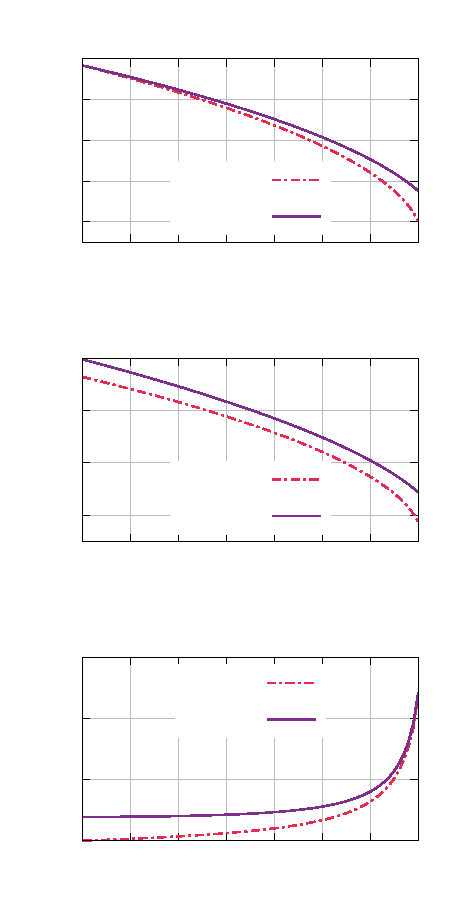
\includegraphics[width={216.00bp},height={432.00bp}]{../tex/ideal-vs-non-ideal-inc}}%
    \gplfronttext
  \end{picture}%
\endgroup
\end{document}
